\subsection{Translating the partitioned code}
\paragraph{Generating equivalent code}
The most basic idea for translating the now partitioned basic blocks is to have a fixed association that maps every instruction in the guest ISA to a sequence of instructions native to the host.

The quality of the code, that can be generated here, strongly depends on the properties of the host and guest architectures in question.
Difficulties can arise due to differences in the instruction operand formats and the types of instruction set architectures the DBT is dealing with.

In our case, as outlined in section~\ref{sec:isa-cmp}, challenges stem from the fact that we are translating code from a load-store architecture using a three-operand instruction format into a register-memory architecture in which (generally) one of the source operands is also the implicit destination operand.
This, for example, means that the single arithmetic instruction \texttt{sub~rd,~rs1,~rs2} in RISC--V assembly language generally can not be translated via a single instruction, but rather requires two instructions: moving \texttt{rs1} to \texttt{rd}, then subtracting the value of \texttt{rs2} from \texttt{rd}.

Opportunities for optimisation lie wherever there is a way to shorten the translation's amount of CPU clock cycles, possibly by employing semantically equivalent native instructions that run in a shorter timespan.
The RISC--V pseudo-instructions (as mentioned in section~\ref{sec:isa-cmp}) are also of some help here~\cite[S. 139]{riscvspec}, along with discoverable patterns in the input assembly.
It is clear, for example, that an instruction like \texttt{xori~x10,~x10,~-1} can be directly translated as a \texttt{not x10}, without needing to resort to \texttt{mov} and \texttt{xor}.
The same principle applies to combinations of multiple instructions.
An \texttt{lui~rd,~imm1} followed by \texttt{addi~rd,~rd,~imm2} may for example be translated as directly loading the result of the computation \texttt{imm1~+~imm2} into \texttt{rd}.

\paragraph{Translation procedure} \mbox{}\\
% todo info about translate-parsing-execution time @Johannes
The translator's central element is the transcode loop, which controls both translation and execution:
First, it is checked whether the block to be executed next has already been translated (see \ref{sec:code-cache}), and if it hasn't, translation is started.
The translated block is then executed, and, before returning to the transcode loop, sets the address where program execution should continue.

%todo: formatting @Johannes use \begin{enumerate}
Translation itself is done in two steps: 

1.: Parsing the guest program's code into easy to work with internal instruction representations, until we hit the end of the basic block.

2.: Translation is then done by dispatching the parsed instructions to special single-instruction translator functions, which emit the matching x86-64 code into memory allocated for the block..

When translation of the block is complete, a \texttt{ret} instruction is appended for returning to the translator after execution.


\subsection{Code cache and block handling}
\label{sec:code-cache}
Naturally, the DBT aims to store the translated code in a semi-permanent way, as it is the goal to not have to translate a required section more than once.

For this, we allocate a region of memory reserved for the basic block translations, also called a \textit{code cache}.
Additionally, an index to this memory section is required, since there needs to be a way to quickly reference the blocks residing in the cache and associate them with both the host and guest instruction pointers that identify them during execution.

The efficiency of the index lookup is increased by a translation lookaside buffer (short \textit{TLB}).
This technique, which is also implemented in the CPU for page lookup, reduces lookup time for most recent used code blocks.
% todo info about chaining and optimisations @Johannes

It is possible that this code cache might fill up during the execution of a large guest program.
If it does, there are two different strategies to handle this issue:
One can either invalidate and purge some or all of the blocks currently residing in the cache, or dynamically resize the cache according to the needs of the guest program~\cite[S. 3]{bintrans}.

Purging the entire cache would require the translator to restart translation on older blocks that might be needed again, introducing a performance overhead that needs to be weighed against the higher memory usage of enlarging the cache.

On the other hand, selective deletion of some of the blocks in the cache is very difficult due to optimisations taken in the context of chaining.
As any chained jumps located in another cached block are dependent on the target block residing in the cache, the target's removal would invalidate these jumps.
It would thus only be possible to either remove all blocks with jump references to the candidate up for removal, or to leave all blocks with jump references in the cache altogether.

\subsection{Register handling and context switching}
\label{sec:context-switch-reg-handle}

\subsubsection{Handling of guest registers}
\label{sec:reg-handle}
As outlined in section~\ref{sec:isa-cmp}, the RISC--V and x86--64 architectures have differing amounts of general purpose registers.
In some way, the state of the 32 general purpose registers \texttt{x1}\footnote{\texttt{x0} is hardwired to a constant zero. All reads will return 0, all writes will be ignored. Hence, this register needs special handling in the DBT, as there is no equivalent construct on x86--64.} to \texttt{x31} and the \texttt{pc} needs to be stored and available to the translations of the identified basic blocks.

As x86--64 only provides 16 general-purpose registers (\texttt{rax}--\texttt{rdx}, \texttt{rbx}, \texttt{rbp}, \texttt{rsi}, \texttt{rdi} and \texttt{r8}--\texttt{r15}), it is impossible to directly and statically map all guest registers to native host registers.
Adding to the above, due to the fact that some x86--64 registers have special or implicit purposes in some instructions like \texttt{(i)mul} or \texttt{(i)/div}, care must be taken in choosing the registers that can be used for such a mapping.
Keeping a guest register file exclusively in memory, and loading them into native registers when needed within the translations of single instructions is technically possible, especially in light of x86--64's ability to extensively use memory operands in the instructions.
However, this necessitates a large number of memory accesses for both memory operands in the instructions as well as local register allocation within the translated blocks.
Due to the very large performance gain connected to using register operands instead of memory operands, this is also not feasible at scale~\cite[S. 8f.]{bintrans}.

Accordingly, the solution for this problem would be an approach that employs parts of both of these extremes~\cite[S. 9]{bintrans}.
We utilise the tools we designed to discover the most-used registers in the guest programs, and statically map these to general purpose x86--64 registers.
The remaining operands are then dynamically allocated into reserved host registers inside a single block's translation.
The loaded values are then lazily kept in the temporary registers for as long as possible in order to avoid unnecessary memory accesses.
In case the translator requires a value not currently present in a replacement register, the oldest value is written back to the register file in memory and the now free space is utilised for the requested value.
The final write-backs then need to be performed on the block boundaries.

The most-used registers are relatively invariant in between RISC--V executables and their basic blocks, however it might be the case that a single block in such an executable requires a few unique registers fairly often.
By dynamically allocating these into temporaries and statically mapping the most-used registers in general, we save much overhead otherwise spent on memory access to the register file, but do not unnecessarily occupy native register space with seldom accessed guest registers.

\subsubsection{Context switching during execution}
When the code translated by the DBT is executed, it will behave as if it were an independent x86--64 executable.
With the static register mapping in place, these values will thus need to be loaded before any of the translated blocks are called, and stored back before the execution is returned to the DBT\@.

This is called a \textit{context switch}, as we are switching from the host's program state made up of the current register values to that of the guest.
Evidently, preserving both the host and guest's state during execution is critical for the correct program behaviour.

\subsection{System call handling}
\label{sec:syscall-handling}
System calls are also a very important part of enabling the guest program's execution.
Thus, every ISA must offer some way to switch the execution context in the kernel mode for the system call to be handled.

For RISC--V, the instruction \texttt{ECALL} (for \textit{environment call}, formerly \texttt{SCALL}) handles these requests, with the system call number residing in register \texttt{a7} and the arguments being passed in \texttt{a0} -- \texttt{a6}.

However, the DBT generally cannot just reorganise the guest argument values and system call identifier according the host's calling convention and relay the system call directly.
The RISC--V guest program expects a different operating system kernel than is present natively on the host;
with that, the system call interface also differs~\cite[S. 2f.]{bintrans}.

In order to handle the \texttt{ECALL} instruction correctly, the translator must thus build the translated instruction to call a specific handler routine not too dissimilar from one that may be found in a kernel.
There, system calls that exist natively on the host architecture as well (like \texttt{write} or \texttt{clock\_gettime}) can usually be passed along to the host's kernel directly.

Care must be taken for system calls that would enable the guest to change the state or context of the host -- an \texttt{mmap} into the translator's memory region, for example, or a call to \texttt{exit} -- these calls must be emulated accordingly to prevent these faults.
In cases where the data structure layout used by the kernels differs, the DBT must also perform necessary actions to adapt the formats to each other.
Some system calls may not exist at all on the native architecture of the host, it is up to the DBT to emulate the required functionality~\cite[S. 2f.]{bintrans}.

\subsection{Floating point extension}
\label{subsec:fp_extension}
Floating point support is a vital part of modern processors, enabling fast computation of real world problems like physics simulations.
While a standard C compiler like \textit{GCC}~\cite{gcc-web} is able to emulate floating point arithmetic using integer arithmetic, using the native support of the x86--64 SSE extensions is evidently a lot faster.

The main difficulties (and their resolutions) that arise by using the x86--64 SSE extensions to translate the RISC--V F- and D-extensions are listed below:
\begin{itemize}
    \item \textbf{Register handling} is similar to the integer register management laid out in section~\ref{sec:context-switch-reg-handle}.
            As mentioned before, the RISC--V architecture consists of 32 floating point registers (\texttt{f0}--\texttt{f31}) which can hold a single precision (F-extension) or double precision (D-extension) floating point value, whereas the SSE-extensions only provide 16 registers \texttt{XMM0}--\texttt{XMM15}.
            We utilise the tools we designed to discover the most-used registers in the guest programs, and statically map these to x86--64 SSE registers \texttt{XMM2}--\texttt{XMM15}.
            One could use the same dynamic mapping approach for the remaining registers as is being used for general purpose registers, but for simplicity reasons registers \texttt{XMM0} and \texttt{XMM1} are reserved for use as replacements and missing registers are loaded into them from memory temporarily.
    \item \textbf{Missing equivalent SSE instructions} can lead to a huge instruction overhead, as emulation often needs to use bit manipulation operations instead.
            For this constants or masks need to be loaded in from either memory or the general purpose registers because the SSE extensions do not support immediate operands.
            The instructions that need to be emulated are unsigned conversion instructions e.g.~\texttt{FCVT.WU.S}, sign-injection instructions e.g.~\texttt{FSGNJ.S}, compare instructions e.g.~\texttt{FEQ.S}, fused multiply-add instructions e.g.~\texttt{FMADD.S} and the \texttt{FCLASS.S} instruction that classifies a floating point value.
            These instructions are not supported by the SSE extension natively.
			One could use the FMA--extension~\cite[S. 141]{intel2017man} to implement the fused multiply-add instructions natively, but these instructions require AVX, which is not generally available on x86--64 hardware.
            As an implementation reference for these instructions, the assembly generated by GCC was used.
    \item \textbf{Rounding modes} are handled differently in the RISC--V architecture, as the rounding mode can be set individually for every instruction.
            The rounding mode of the SSE extension however is controlled by the state of the \texttt{MXCSR} control and status register.
            Thus in case a instruction with explicit rounding mode is encountered, the rounding mode is temporarily changed in the \texttt{MXCSR} register.
    \item \textbf{Exception handling} in RISC--V is realized by reading the \texttt{fcsr} floating-point control and status register, traps are not supported.
            The CSR instructions used to read this register are thus emulated to instead read and translate the \texttt{MXCSR} exception flags.
            x86--64 exceptions are meanwhile disabled by masking them in the \texttt{MXCSR} register.
\end{itemize}


\subsection{Optimisations}
\label{sec:optimise}

\subsubsection{Recursive jump translation}
\label{sec:recursive_translation}
Returning from translated guest code to the translator's main transcode loop comes with big performance penalties.
These are imposed by the first context switch, code cache lookup, and second context switch necessary for starting execution of the next basic block.
To avoid these negative performance impacts, we employ the method of recursive translation: When the parser arrives at an unconditional jump, translation of the jump target is started recursively.
That way, the jump target will always be translated before the jump itself.
Because this means that the jump target's host code address is now already known at translate time, we can emit a direct jump to the target block instead of needing to return to the transcode loop.
The blocks containing jump and target are thereby chained.

\subsubsection{Retroactive block chaining}
\label{sec:chaining}
Translation in general is done lazily.
This especially applies to the handling of conditional jumps, as it is nearly impossible to know at parsing time whether a branch will actually be taken or not.
In cases where the translated conditional jump is not taken during execution, translating the target would cause unnecessary overhead.
For that reason, we do not recursively translate conditional jumps.

If the translator reaches a branch, its two sides can only be chained if the target block has already been translated and its host code address is known.
If that is not the case, the target can instead be chained retroactively after the respective side of the branch is first taken: Following translation of the target block, the branch's host code is modified to jump to the targets now known address directly, instead of returning to the transcode loop.
Further cache lookups and context switching are thus avoided for this branch.

\begin{figure}[h]
	\begin{center}
		\begin{subfigure}[b]{\textwidth}
			\centering
			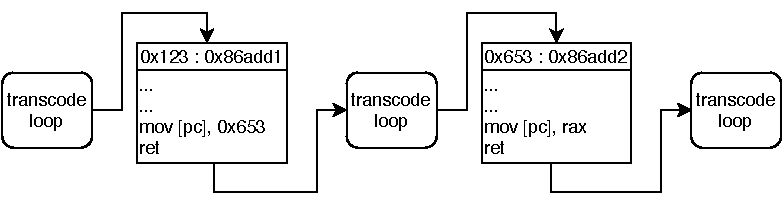
\includegraphics[width=0.8\textwidth]{media/chaining-unchained.pdf}
			\caption{before chaining}
		\end{subfigure}
		\begin{subfigure}[b]{\textwidth}
			\centering
			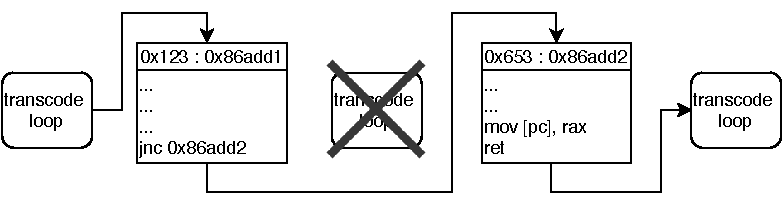
\includegraphics[width=0.8\textwidth]{media/chaining-chained.pdf}
			\caption{after chaining}
		\end{subfigure}
	\end{center}
	
	\caption[Block chaining illustration]%
	{An illustration of retroactive block chaining.}
\end{figure}


\subsubsection{Return address stack}
\label{sec:return-address-stack}
Dynamic jumps can not be statically chained, because their target address may vary.
Still, there is potential for optimisation, as the majority of dynamic jumps found in a typical program are function returns.
By keeping track of function calls, it is possible to predict the return addresses.
In order to do so, we use a stack holding entries for the calls' respective return addresses, that consist of pairs containing both the guest return address and its corresponding host code address.
The stack is implemented as a ring buffer to prevent over- and underflow.

Calls are first detected at parsing time and have their return targets recursively translated.
The call's then emitted host code will push its return address pair onto this stack at every execution without having to leave guest context. %todo simplify sentence structure
Following dynamic jumps will compare their target address with the value in the top stack entry, and, if it matches, pop the address pair and jump to the target block directly, thus avoiding having to return to the transcode loop.
In case of a mismatch the stack will not be changed and control is handed back to the host.


\subsubsection{Macro operation fusion by pattern matching}
\label{sec:pattern-matching}
As RISC--V is a RISC and x86--64 a CISC architecture, programs often need more instructions on RISC--V than on x86--64 to achieve the same effect.
We employ a technique known as macro operation fusion to translate specific patterns of RISC--V instructions into shorter, equivalent x86--64 code, thereby increasing the generated code's performance.
The pattern matcher will detect these patterns after parsing, and replace them with special pseudo-instructions, whose translator functions then emit the corresponding sequence of x86--64 instructions at translate time.

Care must be taken when defining the patterns, as instructions in the pattern might set other register values as a side-effect.
These side-effects must be preserved when replacing the instruction sequences, as later instructions might or might not rely on these values being set correctly.
Thus, either the emitted x86--64 code has to set these registers as well, or the pattern has to only be applicable if no such writes into later used registers occur, thereby constraining the register usage in the instruction combination.
An exemplary excerpt from the patterns we implemented is shown by table~\ref{tab:patterns-table}.

\begin{table*}[t]
	\centering
	\ttfamily
	\small
	\makebox[\textwidth][c]{
	\begin{tabular}{ll}
		\toprule
		LUI r1, imm;\ LW r2, imm(r1);\ ADDI r2, r2, imm;\ SW r2, imm(r1); & ADD m32, imm32\\
		LUI r1, imm;\ LD r2, imm(r1);\ ADDI r2, r2, imm;\ SD r2, imm(r1); & ADD m64, imm32\\
		AUIPC r1, imm;\ ADDI r1, r1;\ & MOV r64, imm64\\
		AUIPC r1, imm;\ LW r1, imm(r1);\ & MOVSX r64, m32\\
		AUIPC r1, imm;\ LD r1, imm(r1);\ & MOV r64, imm64\\
		SLLI r1, r1, 32;\ SLRI r1, r1, 32;\ & MOV r32, r32\\
		ADDIW r1, r1, imm;\ SLLI r1, r1, 31;\ SRLI r1, r1 32;\ & ADD r32, imm32\\
		\bottomrule
	\end{tabular}
	}
	\caption[Patterns used for macro-op-fusion]%
	{Some examples of patterns currently fused by the translator, the last five taken from the RISC--V emulator project rv8~\cite{clark2017rv8}.}
	\label{tab:patterns-table}
\end{table*}















